% ============================================================================
\section{Practical guidance for an attitude-rate-limited TVC lander}\label{sec:practice}
% ============================================================================
\emph{This section reports an algorithm and numerical evidence. Its theorem-level ingredients are \cref{thm:C6}, \cref{thm:CU}
and the elementary claims listed below. Convergence of the outer loop is not proved.}

The theory says where the nonconvexity lives (the attitude profile, \cref{thm:CU}) and what is exactly convex (the problem for a
given attitude, \cref{thm:C6}). The planner below is built on that split. It was implemented for the motivating vehicle and
compared with the current flight guidance \pnote{solver/README.md, RESULTS.md, CLAIMS.md}.

\subsection{Planner B: attitude-aware convex guidance}
The attitude variable is the body angular acceleration $\alpha(t)$ (pitch and yaw), piecewise linear in time, so the gimbal angle
never jumps. With zero roll rate and axisymmetric inertia, the body rate is exactly linear in $\alpha$ (the gyroscopic term
vanishes), and the torque balance of \cref{thm:C6} fixes the lateral thrust, $T_x=-(J_t/L)\alpha_y$, $T_y=(J_t/L)\alpha_x$. The only
remaining control is the axial thrust $T_a(t)$.
\begin{enumerate}[leftmargin=*,itemsep=2pt]
\item \emph{Warm start.} Solve the 3-DOF problem, then fit a smooth attitude profile whose nose follows the 3-DOF thrust direction.
\item \emph{Exact inner solve.} For the fixed attitude profile, solve the SOCP in $T_a$. By \cref{thm:C6} this is the exact
problem, with no relaxation: throttle and gimbal limits become intervals in $T_a$, and the dynamics are affine in $T_a$.
\item \emph{Attitude step.} Linearize only the effect of an attitude change on the thrust direction and solve one convex
trust-region problem in $(\alpha,T_a)$. The minimum-thrust bound is replaced by its tangent plane, which is a safe inner
approximation (Cauchy--Schwarz).
\item \emph{Accept or shrink.} Re-run the exact inner solve at the new attitude. Accept if the merit (fuel plus terminal-defect and
constraint penalties) decreases sufficiently; otherwise shrink the trust region. \emph{Every accepted iterate is an exact solution
of the true dynamics for its attitude}, so the loop can be stopped at any time.
\item \emph{Certificate.} Check the returned plan, not the optimizer, against the physical limits on an $8\times$ finer grid
(throttle $400$--$1000$~N, exact gimbal angles within $\pm15^\circ$, gimbal rate $\le100^\circ$/s, throttle rate, tilt, glide slope,
touchdown defects). Then replay it open loop through a full quaternion rigid-body model, which must land within 5~cm. Fly it
only if it passes.
\end{enumerate}
Planning uses margins inside the physical limits (throttle $440$--$920$~N, gimbal $10^\circ$). Gimbal-rate limits enter as linear sufficient
conditions on node-to-node thrust changes. With $B=\omega_g T_{\rm floor}h$, $t=\tan\delta_p$, $T_z\ge T_{\rm floor}$ and $|T_x|,|T_y|\le tT_z$,
the planner imposes the \emph{pair}
\[
|\Delta T_x|+t|\Delta T_z|\le B\quad(\theta\text{ axis}),\qquad |\Delta T_y|+t|\Delta T_z|\le B\quad(\phi\text{ axis}),
\]
and the pair implies both gimbal-angle rates are at most $\omega_g$. Formalization caught an error here. The originally stated
stand-alone justification for the $\phi$ axis is false: it misses the $\dot T_x$ term, and a counterexample exists. The pair
actually imposed is nevertheless a valid sufficient condition, so no code change was needed.
\begin{todobox}[{(lean-n): Lean status of solver claims N1--N7}]
% CLAIMS: solver/CLAIMS.md N1-N7 (elementary; being formalized by lean-n)
The elementary solver claims are being formalized by [lean-n]: conservative gimbal box (N1), the gimbal-rate pair above (N2),
throttle-slew bound (N3), chord bound (N4), direction-acceleration bound (N5), linear body-rate dynamics (N6), and the 3-DOF lower
bound (N7). \emph{To fill in:} their Lean names and status.
\end{todobox}

\subsection{Results (numerical evidence)}
Comparisons: \textbf{A}, a faithful re-implementation of the flight 3-DOF LCvx; \textbf{C}, 3-DOF LCvx with SOC-representable
thrust-rate limits; \textbf{D}, IPOPT on the full quaternion rigid body (multistart); and \textbf{LB}, the 3-DOF relaxation at the same
$t_f$. Every flyable plan is feasible for the 3-DOF relaxation, so LB is a lower bound, up to its discretization, which is not
bounded rigorously.
\begin{itemize}[leftmargin=*,itemsep=2pt]
\item \emph{Open loop, 8 in-air scenarios} (\cref{fig:openloop}). Every B plan passed the certificate (replay landing within
$0.7$~mm). B is within $0.012\%$ of the best IPOPT optimum (mean $0.005\%$) and at most $0.85\%$ above LB (mean $0.34\%$), so it is
within 1\% of the 6-DOF optimum at that $t_f$. Without attitude iterations (warm start plus one inner solve), only 1 of 8 plans is
certified. C is infeasible at B's $t_f$ in all 8 scenarios; at its own minimum $t_f$ it uses $3.9$--$12.6\%$ more fuel. A's plans
are not flyable: 3 of 8 deliver 296--305~N on the ``400~N'' arc, and they demand instantaneous thrust re-pointing.
\item \emph{Closed loop} (6-DOF plant with wind, gusts, thrust noise, $5\%$ Isp error, gimbal misalignment; common tracker; 1~Hz
replans; success means touchdown $\le1$~m/s, lateral error $\le1$~m, tilt $\le5^\circ$). In-air descents (40 runs): A $28\%$, C $95\%$, B
$100\%$, with median touchdown speeds $2.42$, $0.48$ and $0.20$~m/s (\cref{fig:mcinair}). Pad hops (30 runs): A $0\%$, C $100\%$ at $+23\%$
fuel, B $97\%$ (the one failure skimmed the altitude floor; that is a formulation issue for hops). B's solver time per replan
averaged 0.2--0.4~s, with 9--60 small SOCPs per plan.
\item \emph{The impossibility, visible in practice.} On a grid of 20 pad-hop targets (launch speeds 5--7~m/s, landing offsets
0--6~m, $t_f=4$~s), the 3-DOF relaxation and the flight LCvx report ``optimal'' at all 20. Neither B nor IPOPT finds a flyable plan
at 11 of them: all 8 targets with launch speed $\ge6.5$~m/s, plus 3 targets 6~m away. B and IPOPT agree on feasibility in all 20
cells, and on fuel within $0.3\%$ where both find a plan. ``No IPOPT solution'' is not a proof of infeasibility, but this is exactly
the false-feasibility failure mode Theorem~A predicts for any uniform relaxation (\cref{cor:A}).
\end{itemize}

\begin{figure}[t]\centering
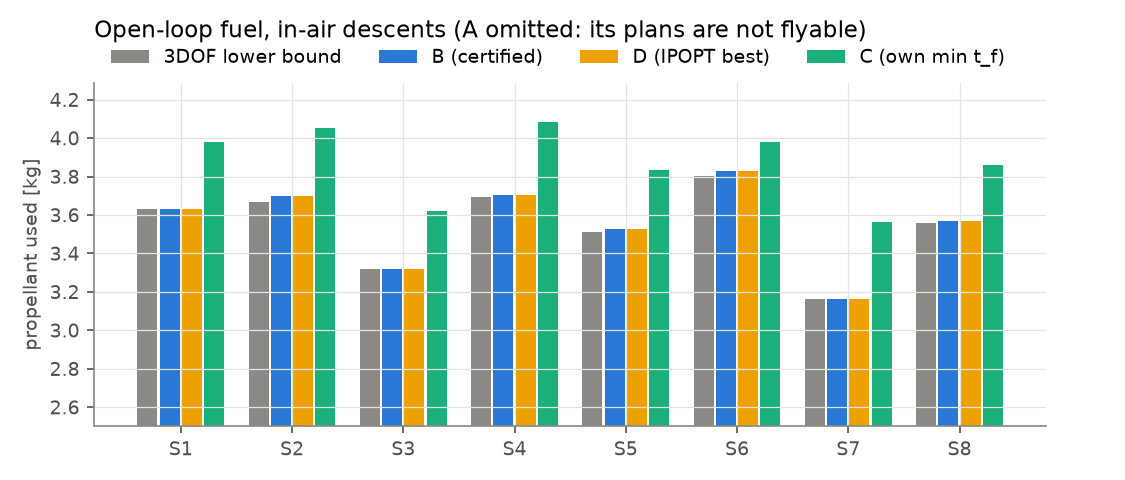
\includegraphics[width=.9\linewidth]{figures/openloop_fuel.png}
\caption{Open-loop fuel for 8 in-air descents: 3-DOF lower bound, planner B (certified), best IPOPT 6-DOF multistart, and 3-DOF with
rate limits at its own minimum $t_f$. Baseline A is omitted because its plans are not flyable. Numerical.}\label{fig:openloop}
\end{figure}
\begin{figure}[t]\centering
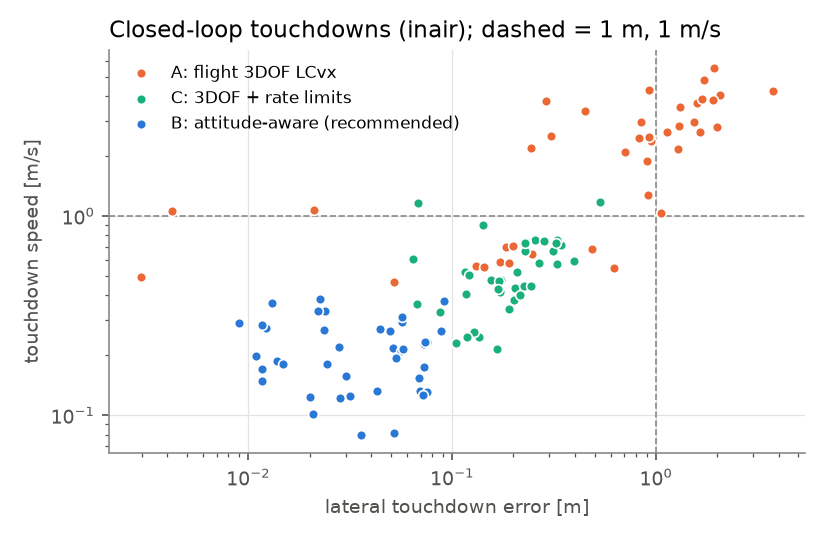
\includegraphics[width=.7\linewidth]{figures/mc_inair_touchdown.png}
\caption{Closed-loop touchdowns, 40 in-air descents per method (dashed lines: 1~m, 1~m/s). Numerical.}\label{fig:mcinair}
\end{figure}

\paragraph{What is and is not guaranteed.} By construction (\cref{thm:C6}), every accepted plan is an exact trajectory of the
planning model for its attitude. The certificate verifies flyability of each returned plan numerically, on a fine grid and by
rigid-body replay, up to floating-point integration error. Not guaranteed: convergence of the outer (SCvx-type) loop to a 6-DOF
KKT point; convergence of the mass fixed point; global optimality (only the gap to LB is bounded); and robustness to plant
mismatch, which is Monte Carlo evidence only.
